\documentclass{article}
\usepackage{graphicx} % Required for inserting images
\usepackage[T2A]{fontenc}
\usepackage[english, russian]{babel}

\setlength\parindent{1.5em}


\title{Домашнее задание 3}
\author{Андрей Зотов}
\date{Май 2023}
\begin{document}

\maketitle

\section*{Задача 1}
{\bf Ответ:}
\begin{itemize}
\item a) Максимальная длина простого цикла в графе $G$ равняется 4. Всего имеется 16 различных простых циклов максимальной длины 4.
\item б) Да, верно.
\item в) Минимум 2 ребра надо удалить из графа $G$, чтобы он стал несвязным.
\end{itemize}
{\bf Решение.} а) Всего в графе $G$ имеется 6 различных подграфов, которые образуют простые циклы: $ABD, DBC, ABCD, CEH, HEF, CEFH$. Два из этих подграфов - $ABCD, CEFH$ - самые большие и образуют простые циклы длины 4. Каждый из подграфов длины 4 дает 8 разных простых циклов (стартовую вершину цикла можно выбрать 4-мя способами и направление 2-мя способами $\Rightarrow 4 * 2 = 8$ разных простых циклов получается из одного подграфа). Таким образом в графе $G$ имеется 16 разных простых циклов максимальной длины 4.
\par
б) Не трудно заметить, что, во-первых, граф $G$ связный, а во-вторых, для любого ребра графа $G$ существует цикл (а иногда и не один), в который входит это ребро. А т.к. удаление любого ребра из цикла не может нарушить связность графа, который содержит этот цикл, то удаление любого ребра не может нарушить связность графа $G$.
\par
в) Учитывая п. б) искомое минимальное кол-во ребер не может быть меньше двух, при этом если из графа $G$ удалить 2 ребра, например $CB$ и $CD$, то граф распадется на 2 компоненты связности, т.е. 2 и есть искомое минимальное кол-во ребер.
\section*{Задача 2}
{\bf Ответ:} 200 дорог в государстве.
\\
\\
{\bf Решение.} Пусть города будут множеством вершин $V$, а дороги множеством ребер $E$ некоего графа $G$. Тогда по лемме о рукопожатиях $\sum_{v_i \in V}\deg{v_i} = 2 |E|$. При этом по условию задачи $\forall v_i \in V\ \deg{v_i}=4$ и $|V|= 100$, т.е. $4*100=2|E|$. Поэтому кол-во дорог будет $|E|=200$.
\section*{Задача 3}
{\bf Ответ:}
\begin{itemize}
\item a) Можно.
\item б) Нельзя.
\end{itemize}
{\bf Решение.} a) Рассмотрим картинку а) как граф $G$, где точки пересечения - это вершины графа $G$, а дуги это ребра графа $G$. Получившийся граф $G$ очевидно связен. Тогда требование задачи будет выполнимо тогда и только тогда, когда у графа $G$ существует эйлеров путь. Т.к. все вершины графа $G$ имеют четную степень 4, то по критерию эйлеров путь существуют (причем он является также эйлеровым циклом).
\par
Хотя критерий верен и для графов с кратными ребрами мы без ущерба для рассуждения можем избавиться от кратных ребер в $G$, добавив две вершины ($J$ и $K$) степени 2 на крайние левую и правую дуги нашей фигуры (на наличие эйлерова цикла, очевидно, это не повлияет). В итоге имеем граф $ABCDEFGHJK$, который изображен на картинке ниже. Эйлеров цикл (т.е. путь, вдоль которого можно вести карандаш, не отрывая от бумаги и проходя по каждой линий по одному разу) в нем будет, например, таким: 
$$K,B,D,H,J,G,F,H,G,E,C,D,F,E,A,B,C,A,K$$
\\
{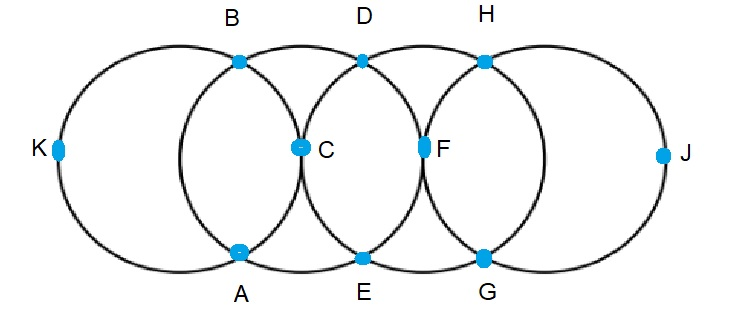
\includegraphics[scale=0.3]{img/img1.jpg}}
\par
б) Аналогично а) рассмотрим картинку б) как связный граф и заметим, что в нем будет 8 вершин нечетной степени 3 (см. рисунок ниже). Поэтому согласно критерию (в графе должно быть не больше двух вершин нечетной степени), в таком графе эйлеров путь не существует, а значит и нарисовать картинку б), не отрывая карандаш от бумаги и проходя по каждой линии по одному разу невозможно.
\\
{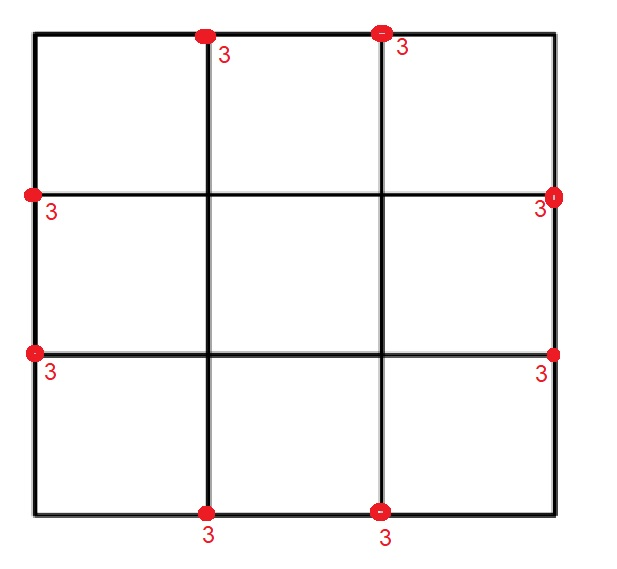
\includegraphics[scale=0.2]{img/img2.jpg}}
\section*{Задача 4}
{\bf Ответ:} одна вершина имеет степень 3.
\\
\\
{\bf Решение.} Т.к. у дерева ровно три вершины имеют степень 1, то в дереве не существует вершин, у которых степень больше 3-х. Докажем это.
\par
Допустим это не так, пусть в дереве есть вершина $A$, из которой выходит $n>3$ ребер. Если из исходного дерева удалить вершину $A$ и все ребра, которые из нее выходят, то образуются $n$ подграфов, каждый из которых тоже дерево (т.к. подграф дерева - это дерево).  Все эти поддеревья не связаны между собой, т.к. иначе существовал бы цикл в исходном дереве, проходящий через вершину $A$, что невозможно (т.к. в дереве нет циклов). 
\par
В каждом из $n$ изолированных друг от друга поддеревьев либо существует хотя бы один лист (т.е. вершина со степенью 1), либо поддерево состоит из одной единственной вершины - в обоих случаях такие вершины имеют степень 1 в исходном дереве. Поэтому в исходном дереве существует минимум $n > 3$ листьев, а это невозможно, т.к. листьев по условию ровно 3. Противоречие. 
\par
Таким образом в рассматриваемом дереве у вершин могут быть степени только 1, 2 или 3.
\par
Если в рассматриваемом дереве $x$ - кол-во вершин степени $3$ и 3 вершины степени 1, тогда кол-во вершин степени 2 будет $2022-3-x$.  При этом число ребер дерева будет $|E|=|V|-1 = 2022 - 1 = 2021$  и по лемме о рукопожатиях имеем:
$$2*|E| = 2*2021 = 4042 = \sum_{v_i\in V}\deg{v_i}=1*3+2*(2022-3-x)+3*x$$
Что равносильно
$$3x - 2x + 3+2*2019 = 4042$$
А это в свою очередь равносильно
$$x = 1$$
\par
Таким образом, если такое дерево существует, то в нем ровно 3 вершины степени 1, ровно 2018 вершин степени 2 и ровно одна вершина имеет степень 3. Такой граф действительно существует - его изображение на картинке ниже.
\\
{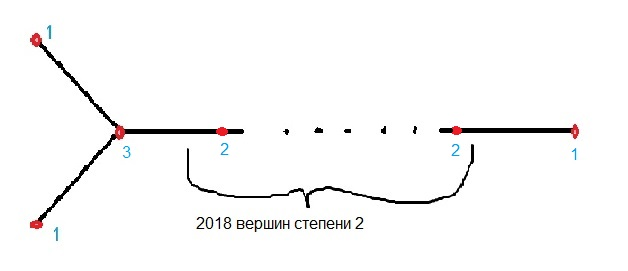
\includegraphics[scale=0.6]{img/img3.jpg}}
\section*{Задача 5}
{\bf Доказательство.} Пусть $G$ исходный граф, $V$ - множество его вершин и $E$ - множество его ребер. Рассмотрим дополнение $\overline{G}$ к графу $G$. Множество вершин дополнения $\overline{G}$ совпадает с $V$, а множество ребер дополнения $\overline{G}$ обозначим $\overline{E}$. Т.к. $|V|=6$ и $|E|=11$, то по определению дополнения $|E\cup\overline{E}|= (\textrm{число ребер в полном графе}\ K_6)=\frac{6*5}{2}=15$ и т.к. $E\cap\overline{E}=\emptyset$, то $|\overline{E}|=15 - |E| = 15 - 11 = 4$. Таким образом дополнение $\overline{G}$ - это граф на 6 вершинах с 4-мя ребрами. 
\par
Покажем, что $\overline{G}$ - не связен. Допустим $\overline{G}$ связен и следовательно у  $\overline{G}$ существует остовное дерево, в котором не более 4-х ребер и 6 вершин. Но у дерева с 6 вершинами должно быть ровно 5 ребер. Противоречие. Следовательно, $\overline{G}$ не связен. 
\par
Т.к. граф и его дополнение не могут быть не связными графами одновременно (пример 3.8), то $G$ связен. Что и требовалось.
\section*{Задача 6}
{\bf Ответ:} нельзя.
\\
\\
{\bf Решение.} Обозначим все поля доски $3\times3$ как принято в шахматах - от $a1$ до $c3$ (9 полей). Составим граф, вершины которого будут поля (кроме поля $c2$, т.к., очевидно, ни один конь на это поле никогда не попадет), а ребра будут возможные ходы коня с данного поля. Тогда получим такой граф:
\\
{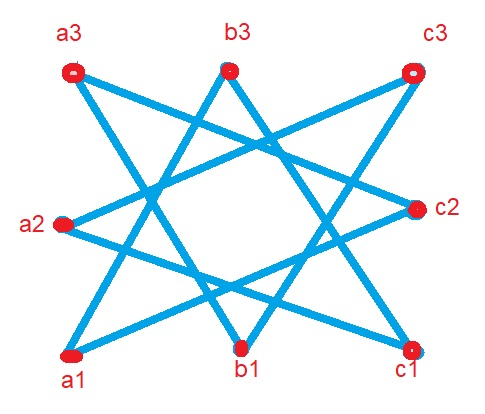
\includegraphics[scale=0.3]{img/img4.jpg}}
\\
Как видно $a1,b3,c1,a2,c3,b1,a3,c2, a1$ - простой цикл, при этом этот путь еще и эйлеров цикл. Поэтому этот граф эквивалентен следующему:
\\
{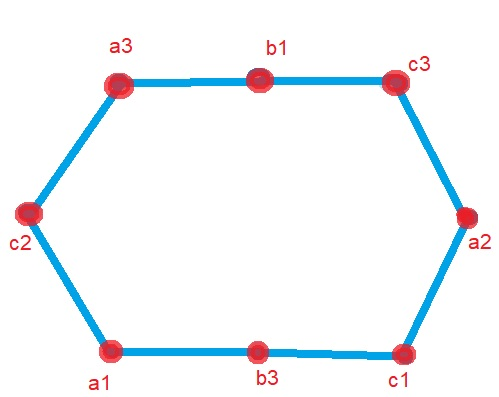
\includegraphics[scale=0.3]{img/img5.jpg}}
\\
Тогда задача состоит в том, что можно ли найти последовательность ходов такую, что белые кони, стартуя с полей $a1,c1$ и черные - с полей $a3,c3$, поочередно двигаясь по ребрам графа, придут на поля $a1,c3$ (белые) и $a3,c1$ (черные). Это невозможно, т.к. с одной стороны как бы ни перемещались кони вдоль ребер графа должна сохраняться последовательность коней ЧЧББ при обходе графа по циклу (иначе в какой-то момент две фигуры будут вынуждены располагаться на одном поле, а это запрещено правилами). А с другой стороны, в конечной позиции имеем последовательность ЧБЧБ при обходе графа по циклу, которую невозможно получить из позиции вида ЧЧББ. Т.е. ЧЧББ  $\not \rightarrow$ ЧБЧБ.
\\
{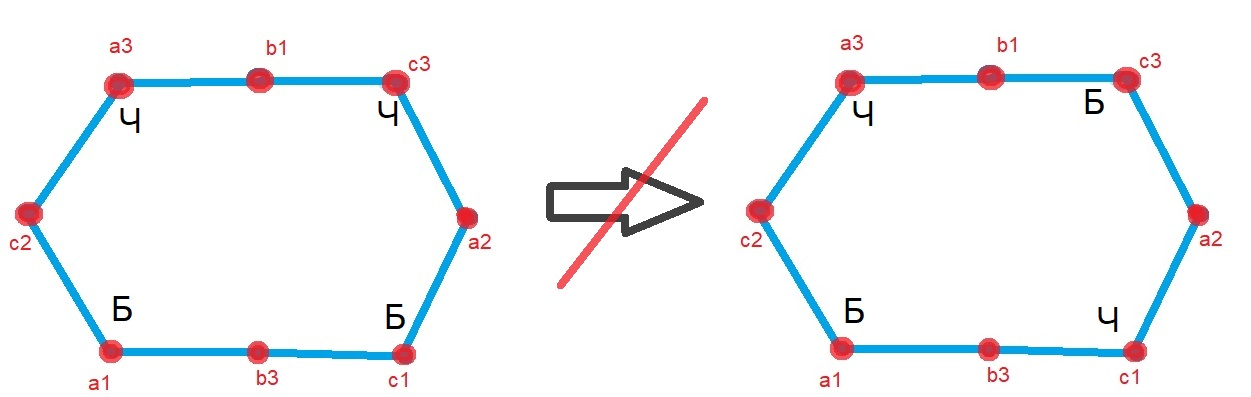
\includegraphics[scale=0.4]{img/img6.jpg}}
\\
P.S. В терминах разрезов можно еще так пояснить, что ЧЧББ  $\not \rightarrow$ ЧБЧБ. Граф в левой части рисунка выше показывает, что какие бы ни делались ходы конями в любой момент существует разрез графа, такой что в одной части графа окажутся все белые кони, а в другой все черные. Однако для графа в правой части такого разреза не существует.
\end{document}
